\subsection{Параметры согласованного фильтра и выходного сигнала}
В этом задании изучаются характеристики согласованных фильтров,
соответствующих каждому из сигналов, рассмотренных в задании №1. Кроме
того, исследуются вид и свойства выходных сигналов. Учитывая, что при
расширении фазового спектра длительность сигнала увеличивается, а при
уменьшении до нуля – укорачивается, в данном задании необходимо
внимательно проследить за укорочением сигнала. Самый короткий и самый
большой по амплитуде он должен получиться при нулевом фазовом спектре

\subsubsection*{Рекомендации по анализу результатов эксперимента}%
\label{ssub:rekomendatsii_po_analizu}

%\begin{itemize}
    %\item[$\checked$] Как коэффициент передачи по амплитуде $\abs{K(\omega)}$ фильтра и
        %фазовые сдвиги $\phi(\omega)$, вносимые фильтром в соответствующую
        %гармонику, связаны с амплитудным и фазовым спектром сигнала?  
    %\item[$\checked$] Какой вид имеет импульсная переходная характеристика согласованного
        %фильтра?

    %\item[$\times$] Как связан выходной сигнал и его амплитудный и фазовый спектр с
    %характеристиками выходного сигнала? Сравнить длительности входного и
    %выходного сигналов.  
    %\item[$\times$] Какой фазовый спектр и база выходного сигнала?
%\end{itemize}





АЧХ $\abs{K(i \omega)}$ и ФЧХ $\varphi (\omega)$ согласованного фильтра связаны с 
амплитудным и фазовым спектром сигнала следующим образом:
\begin{equation}
    \abs{K(i \omega)} = \abs{C_0} \cdot \abs{C_m(i \omega)}, \quad
    \varphi (\omega) = -\varphi_m  -\omega t + arg(C_0),
\end{equation}
где $C_m, \varphi_m $ - амплитудный и фазовый спектры входного сигнала $m(t)$.

Во всех случаях импульсная переходная характеристика фильтра имеет вид зеркально отраженного сигнала, сдвинутого таким
образом, чтобы начало характеристики совпадало с $t=0$.
\begin{equation}
    h(t) = C_0 m(-(t-t_0)) = C_0 m(-t+t_0).
    \label{eq:}
\end{equation}

Сигнал на выходе согласованного фильтра пропорционален функции корреляции первого рода:
\begin{equation}
    M(t) = C_0 \Psi (t_0-t) = \int \limits_{-\infty}^{\infty} C_0 m(t')m(t_0-t+t') \dd t'
    \label{eq:}
\end{equation}

\subsubsection{Прямоугольный видеоимпульс}
Рассмотрим прохождение прямоугольного видеоимпульса через согласованный фильтр. Рассмотрим два случая: длительность $T$
10 и 30 мс. Результаты работы программы приведены соответсвенно но рис. \ref{fig:task_2_1_10} и \ref{fig:task_2_1_30}.
\begin{figure}[H]
    \centering
    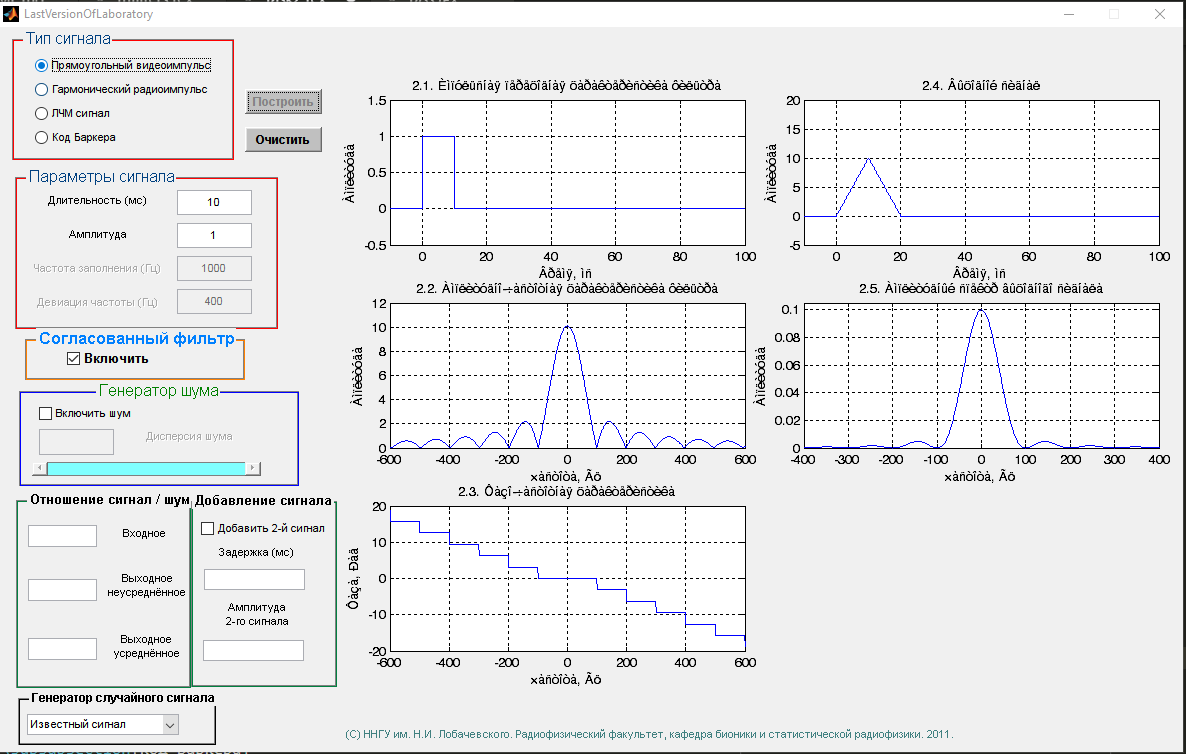
\includegraphics[width=0.9\linewidth]{imgs/task_2/t2s1_10.png}
    \caption{Прямоугольный видеоимпульс, пропущенный через согласованный фильтр, $T = 10$ мс}
    \label{fig:task_2_1_10}
\end{figure}
\begin{figure}[H]
    \centering
    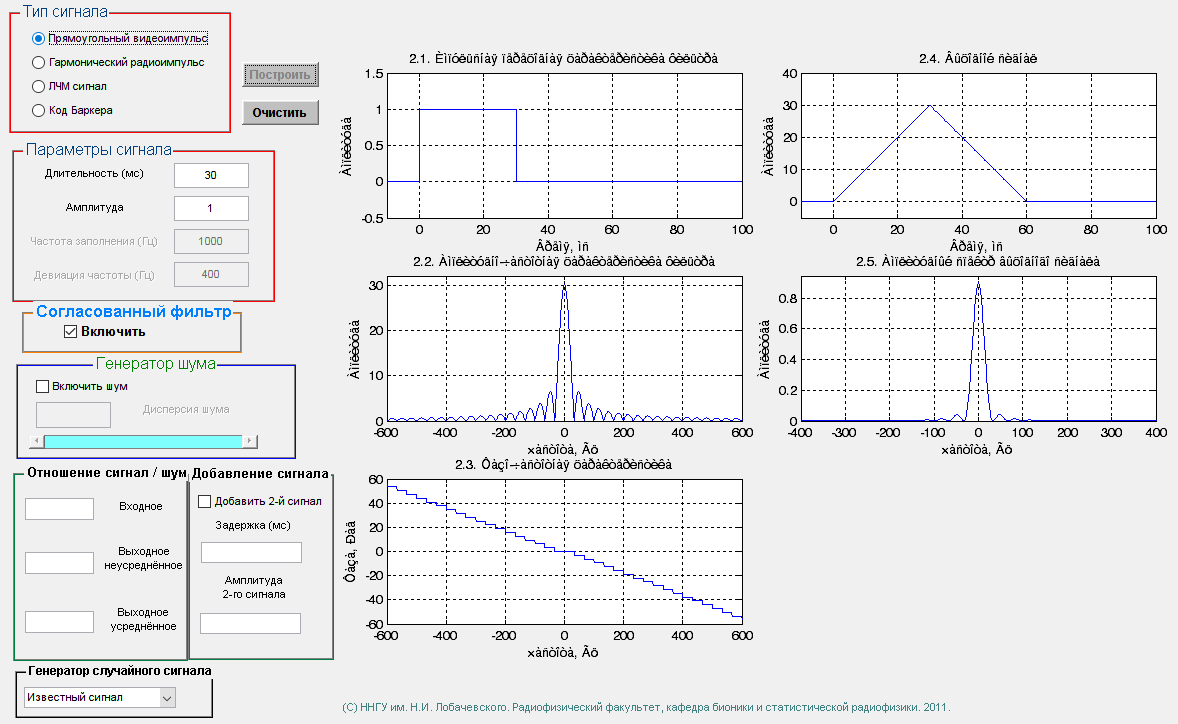
\includegraphics[width=0.9\linewidth]{imgs/task_2/t2s1_30.png}
    \caption{рямоугольный видеоимпульс, пропущенный через согласованный фильтр, $T = 30$ мс}
    \label{fig:task_2_1_30}
\end{figure}

\begin{enumerate}
    \item При увеличении длительности входного сигнала, длительность выходного сигнала также увеличивается, а
    амплитудный спектр выходного сигнала сужается.
    \item Определим базу выходного сигнала. 
    \begin{equation}
        B_{10ms} = T \cdot \Delta f \simeq 20 \cdot 10^{-3} \cdot 90 = 1.8
    \end{equation}
    \begin{equation}
        B_{30ms} = T \cdot \Delta f \simeq 60 \cdot 10^{-3} \cdot 30 = 1.8
    \end{equation}
    База выходного сигнала больше базы входного.
\end{enumerate}


\subsubsection{Прямоугольный видеоимпульс с гармоническим заполнением}
Пропустим через согласованный фильтр радиоимпульс с чатотой заполнения 500 Гц, и длительностью 10 и 30 мс. Результаты
приведены на рис. \ref{fig:task_2_2_10} и \ref{fig:task_2_2_30} соответственно.
\begin{figure}[H]
    \centering
    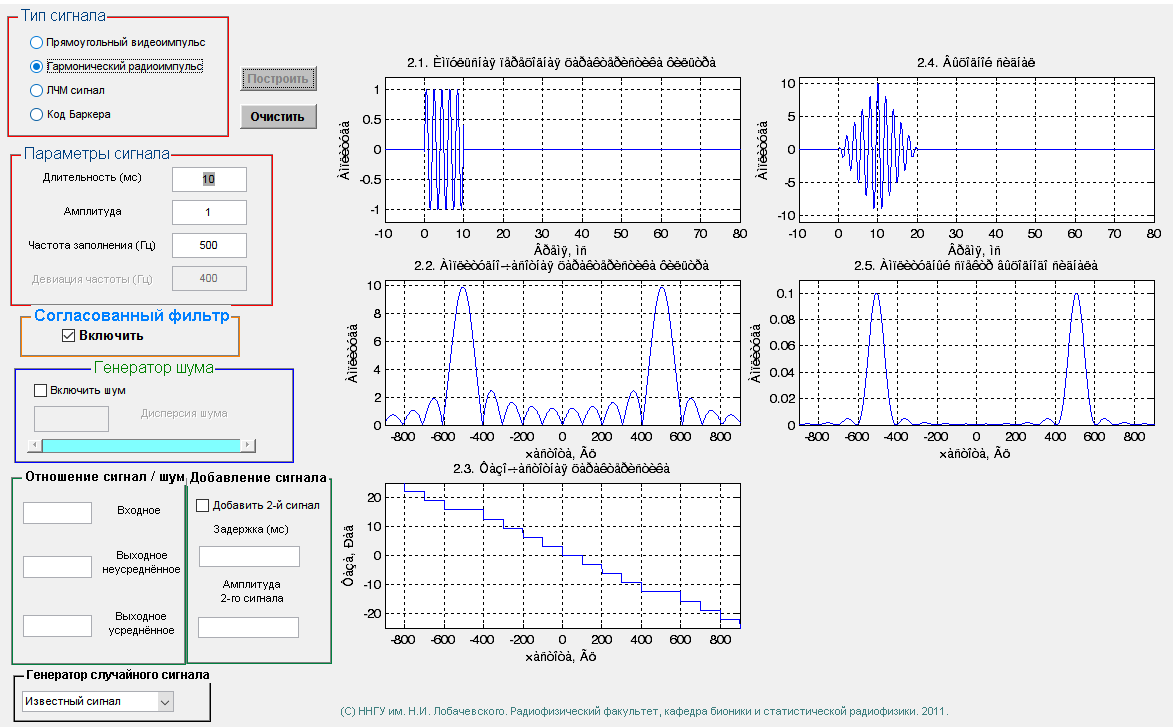
\includegraphics[width=0.9\linewidth]{imgs/task_2/t2s2_10.png}
    \caption{10 мс}
    \label{fig:task_2_2_10}
\end{figure}
\begin{figure}[H]
    \centering
    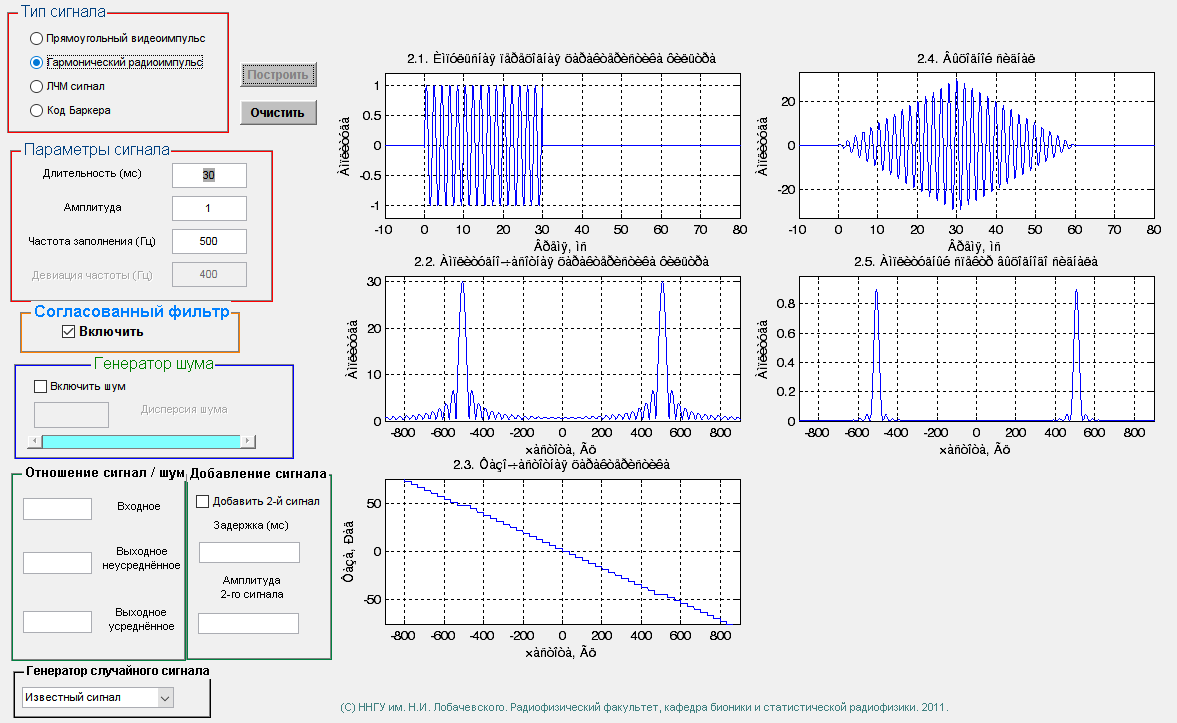
\includegraphics[width=0.9\linewidth]{imgs/task_2/t2s2_30.png}
    \caption{30 мс}
    \label{fig:task_2_2_30}
\end{figure}

Результаты анализа радиоимпульса аналогичны результатам для видеоимпульса:
\begin{enumerate}
    \item При увеличении длительности входного сигнала, длительность выходного сигнала также увеличивается, а
    амплитудный спектр выходного сигнала сужается.
    \item Определим базу выходного сигнала. 
    \begin{equation}
        B_{10ms} = T \cdot \Delta f \simeq 20 \cdot 10^{-3} \cdot 80 = 1.6
    \end{equation}
    \begin{equation}
        B_{30ms} = T \cdot \Delta f \simeq 60 \cdot 10^{-3} \cdot 25 = 1.5
    \end{equation}
    База выходного сигнала больше базы входного.
\end{enumerate}


\subsubsection{ЛЧМ сигнал}
Далее рассмотрим ЛЧМ сигнал. Зададим длительность сигнала 100мс, частоту заполнения 1000 Гц, а
девиацию возьмем равной 500 и 1000 Гц. Результаты приведены на рис. \ref{fig:task_2_3_500} и \ref{fig:task_2_3_1000}
соответственно.
\begin{figure}[H]
    \centering
    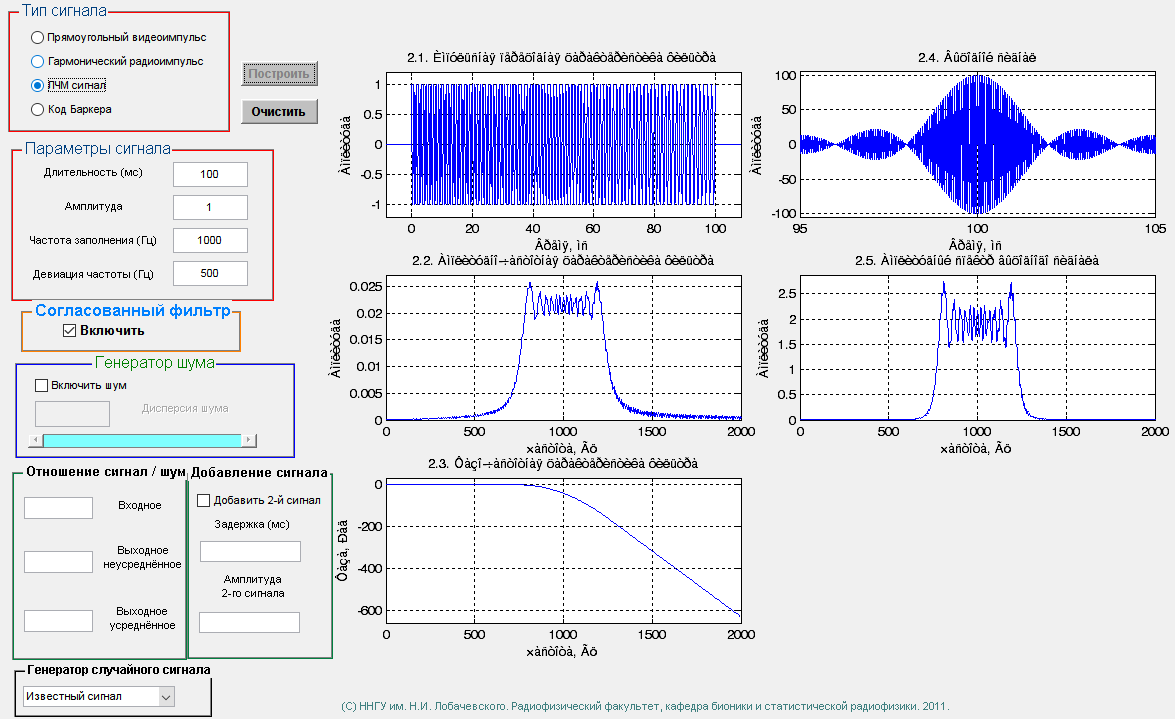
\includegraphics[width=0.9\linewidth]{imgs/task_2/t2s3_500.png}
    \caption{Девиация 500 Гц}
    \label{fig:task_2_3_500}
\end{figure}
\begin{figure}[H]
    \centering
    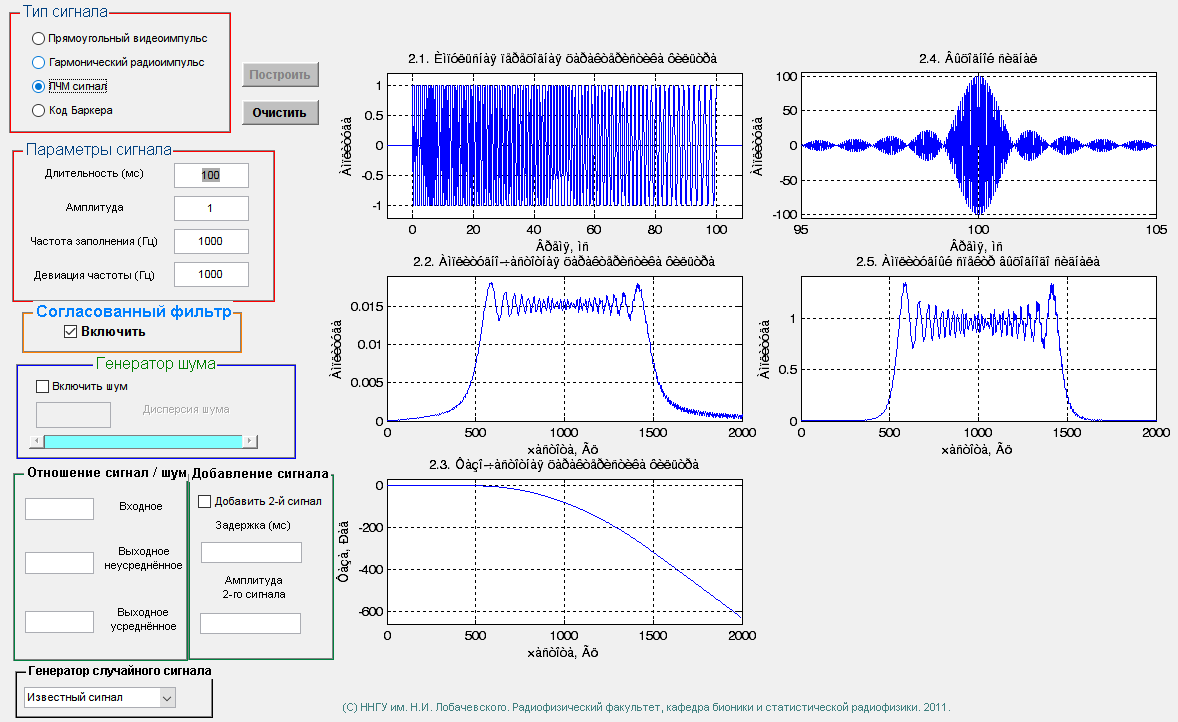
\includegraphics[width=0.9\linewidth]{imgs/task_2/t2s3_1000.png}
    \caption{Девиация 1000 Гц}
    \label{fig:task_2_3_1000}
\end{figure}

Импульсная характеристика перешла в ЛЧМ-колебание с зеркальной по отношению к сигналу модуляцией.
\begin{enumerate}
    \item Сравним длительности входного и выходного сигналов. Эффективная длительность выходного сигнала составляет 4
    мс, при этом она не зависит от длительности входного сигнала. Это происходит из-за сжимающих свойств фильтра, и того
    факта что ЛЧМ сигнал является сложным сигналом. В данном случае он обладает базой $B \simeq 50$, что мы и наблюдаем
    при уменьшении длительность выходного сигнала в $\sim B$ раз.

    При увеличении величины девиации, эффективная длительность выходного сигнала уменьшилась в два раза, составляя 2 мс.
    Амплитудный спектр при этом не изменился.
    \item Определим базу выходного сигнала. 
    \begin{equation}
        B_{500 Hz} = T \cdot \Delta f \simeq 4 \cdot 10^{-3} \cdot 500 = 2
    \end{equation}
    \begin{equation}
        B_{1000 Hz} = T \cdot \Delta f \simeq 2 \cdot 10^{-3} \cdot 1000 = 2
    \end{equation}
    База выходного сигнала меньше базы входного, за счет сильного уменьшения длительности и сохранения спектра.
\end{enumerate}


\subsubsection{Код Баркера}
Далее рассмотрим код Баркера. Зададим длительность сигнала равной 13 с и 26 с.
Результаты приведены на рис. \ref{fig:task_2_4_13} и \ref{fig:task_2_4_26} соответственно.
\begin{figure}[H]
    \centering
    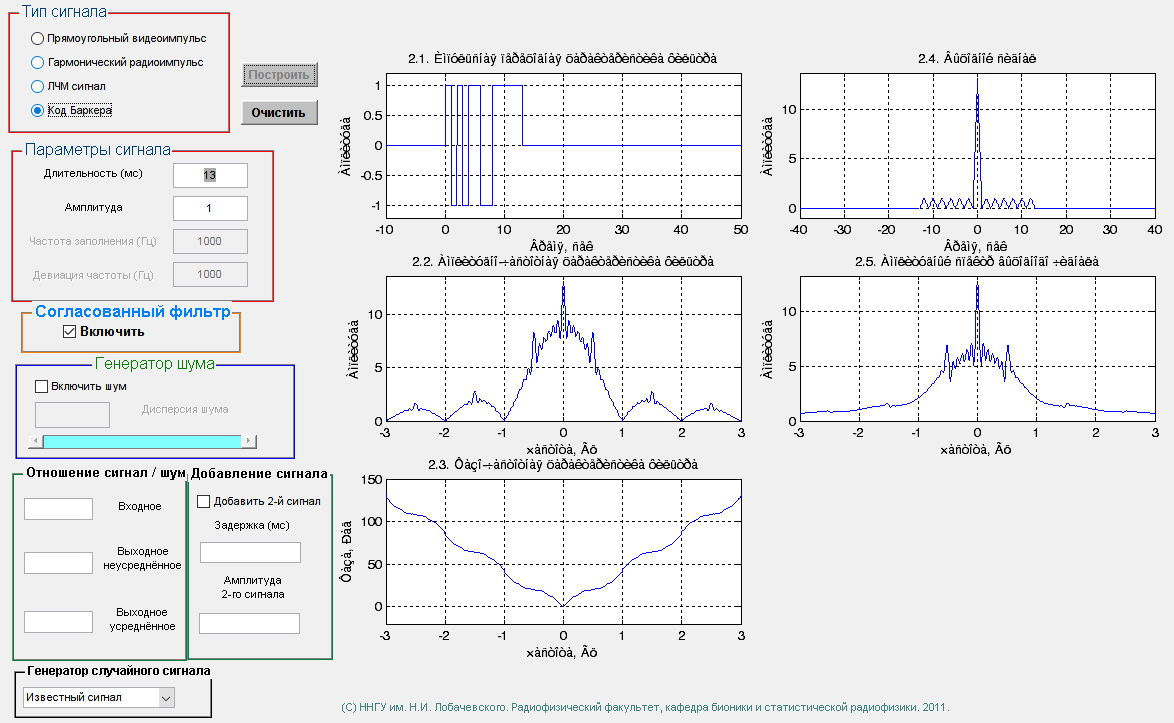
\includegraphics[width=0.9\linewidth]{imgs/task_2/t2s4_13.png}
    \caption{13 с}
    \label{fig:task_2_4_13}
\end{figure}
\begin{figure}[H]
    \centering
    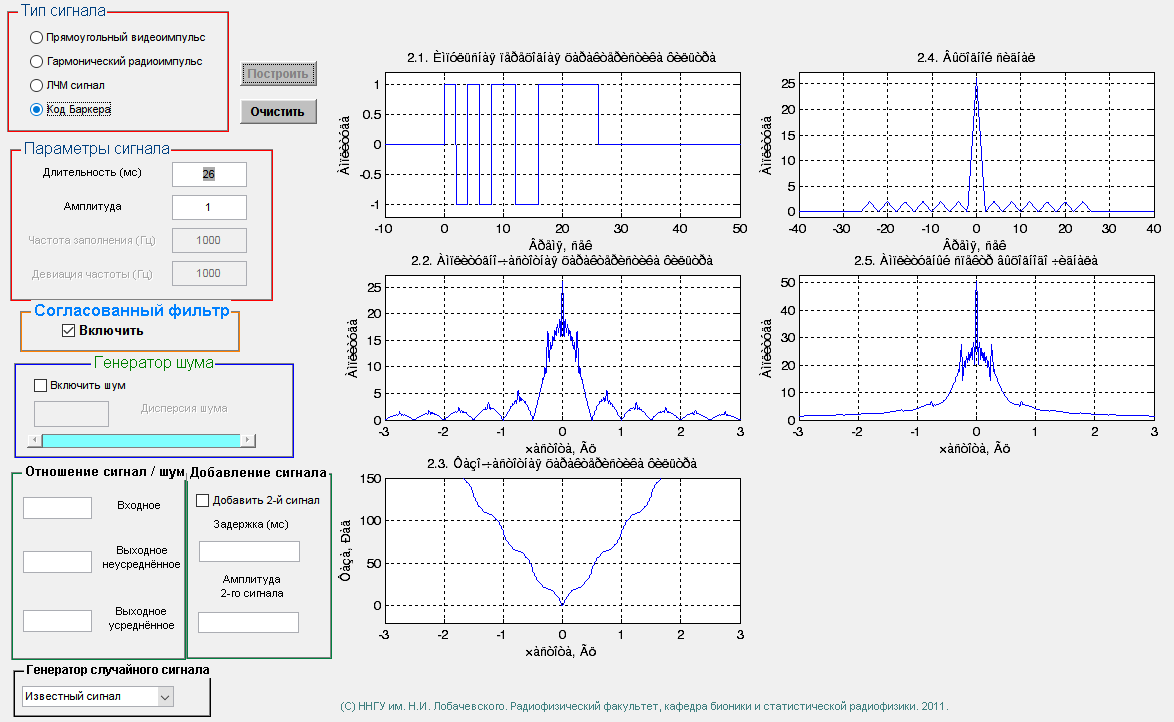
\includegraphics[width=0.9\linewidth]{imgs/task_2/t2s4_26.png}
    \caption{26 с}
    \label{fig:task_2_4_26}
\end{figure}

\begin{enumerate}
    \item При длительности входного сигнала в 13 с, эффективная длительность выходного сигнала составляет
    26 с. При этом при увеличении длительности входного сигнала до 26 с, длительность выходного также увеличилась в два раза.
    \item Определим базу выходного сигнала. 
    \begin{equation}
        B_{13 s} = T \cdot \Delta f \simeq 2 \cdot 26 = 52
    \end{equation}
    \begin{equation}
        B_{26 s} = T \cdot \Delta f \simeq 2 \cdot 52 = 104
    \end{equation}

\end{enumerate}
